\chapter{Requirement Analysis}
\label{ch:requirement-analysis}

This chapter outlines the analytical framework used to determine the needs, roles, and interactions involved in the research project. It defines the stakeholders, scenarios of system usage, and initial user interface concepts for interacting with the EEG-based Motor Imagery (MI) classification platform.


\section{Stakeholder Analysis}
\label{sec:stakeholder-analysis}

Stakeholders in this research include individuals and groups who interact with, contribute to, or benefit from the system developed for EEG-based MI classification using self-supervised learning.

\begin{itemize}
    \item \textbf{Research Students:} Graduate and undergraduate students conducting EEG or BCI-related research who require tools for preprocessing, modeling, and visualizing EEG signals.
    \item \textbf{Academic Advisors and Mentors:} Supervisors who guide the project, evaluate methodologies, and assess results.
    \item \textbf{BCI Researchers:} Specialists in Brain-Computer Interface systems who are interested in integrating the framework into larger research workflows.
    \item \textbf{Collaborative Institutions:} External collaborators or co-authors who may contribute datasets, methods, or validation tools.
\end{itemize}


\section{User Stories}
\label{sec:user-stories}

User stories are derived from research scenarios rather than business objectives.
These help define how each type of stakeholder would interact with the system.

\begin{itemize}
    \item \textbf{As a research student}, I want to upload raw EEG datasets from various MI tasks so that I can run preprocessing and train SSL models.
    \item \textbf{As an academic advisor}, I want to review model performance summaries and confusion matrices so that I can evaluate the effectiveness of the SSL training.
    \item \textbf{As a BCI researcher}, I want to compare the accuracy of traditional supervised models with the SSL framework so that I can determine its viability for cross-subject generalization.
    \item \textbf{As a collaborator}, I want to integrate new datasets into the framework pipeline so that I can validate the model across different data sources.
\end{itemize}


\section{Use Case Diagram}
\label{sec:use-case-diagram}
The system supports various interactions between researchers and the components of the EEG SSL framework. Below is a use case diagram representing primary research activities.


\begin{figure}[H]
    \centering
    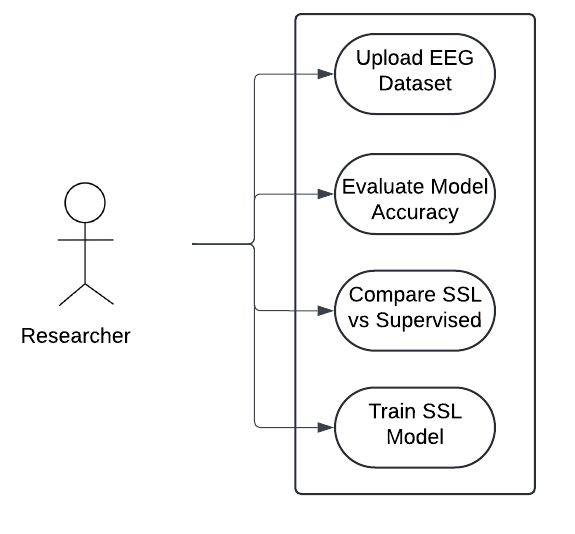
\includegraphics[width=0.85\textwidth]{figures/use-case-diagram-eeg}
    \caption{Use Case Diagram for EEG SSL Framework}\label{fig:figure}
\end{figure}
\newpage

\section{Use Case Model}
\label{sec:use-case-model}

This section outlines key use cases using a brief or casual structure appropriate for a research prototype.

\subsection*{Use Case: Upload EEG Dataset}
\textbf{Type:} Brief
\textbf{Actor:} Researcher
\textbf{Goal:} To upload a raw EEG dataset for preprocessing and model training.

\subsection*{Use Case: Train SSL Model}
\textbf{Type:} Casual
\textbf{Primary Actor:} Researcher
\textbf{Preconditions:} Dataset has been preprocessed.
\textbf{Main Flow:}
\begin{enumerate}
    \item User selects the preprocessed dataset.
    \item User configures SSL model parameters.
    \item System begins training and logs progress.
    \item Upon completion, results are visualized and saved.
\end{enumerate}

\subsection*{Use Case: Evaluate Model Accuracy}
\textbf{Type:} Casual
\textbf{Actor:} Researcher
\textbf{Goal:} To view performance metrics of the trained model.

\subsection*{Use Case: Compare SSL vs Supervised}
\textbf{Type:} Brief
\textbf{Actor:} Researcher
\textbf{Goal:} Compare results of SSL model with a baseline supervised model.
\newpage

\section{User Interface Design}
\label{sec:user-interface-design}

The user interface is designed to support interaction with the model training pipeline, prediction, evaluation, and model comparison.
It aims to simplify research workflows such as dataset selection, preprocessing, training configuration, and performance analysis.

The UI is implemented using HTML and Tailwind CSS for a clean, responsive layout.
Each screen is tailored to specific research tasks, ensuring usability for academic researchers with limited software engineering experience.

The UI is divided into multiple functional views, as shown below:

\begin{figure}[h]
    \centering
    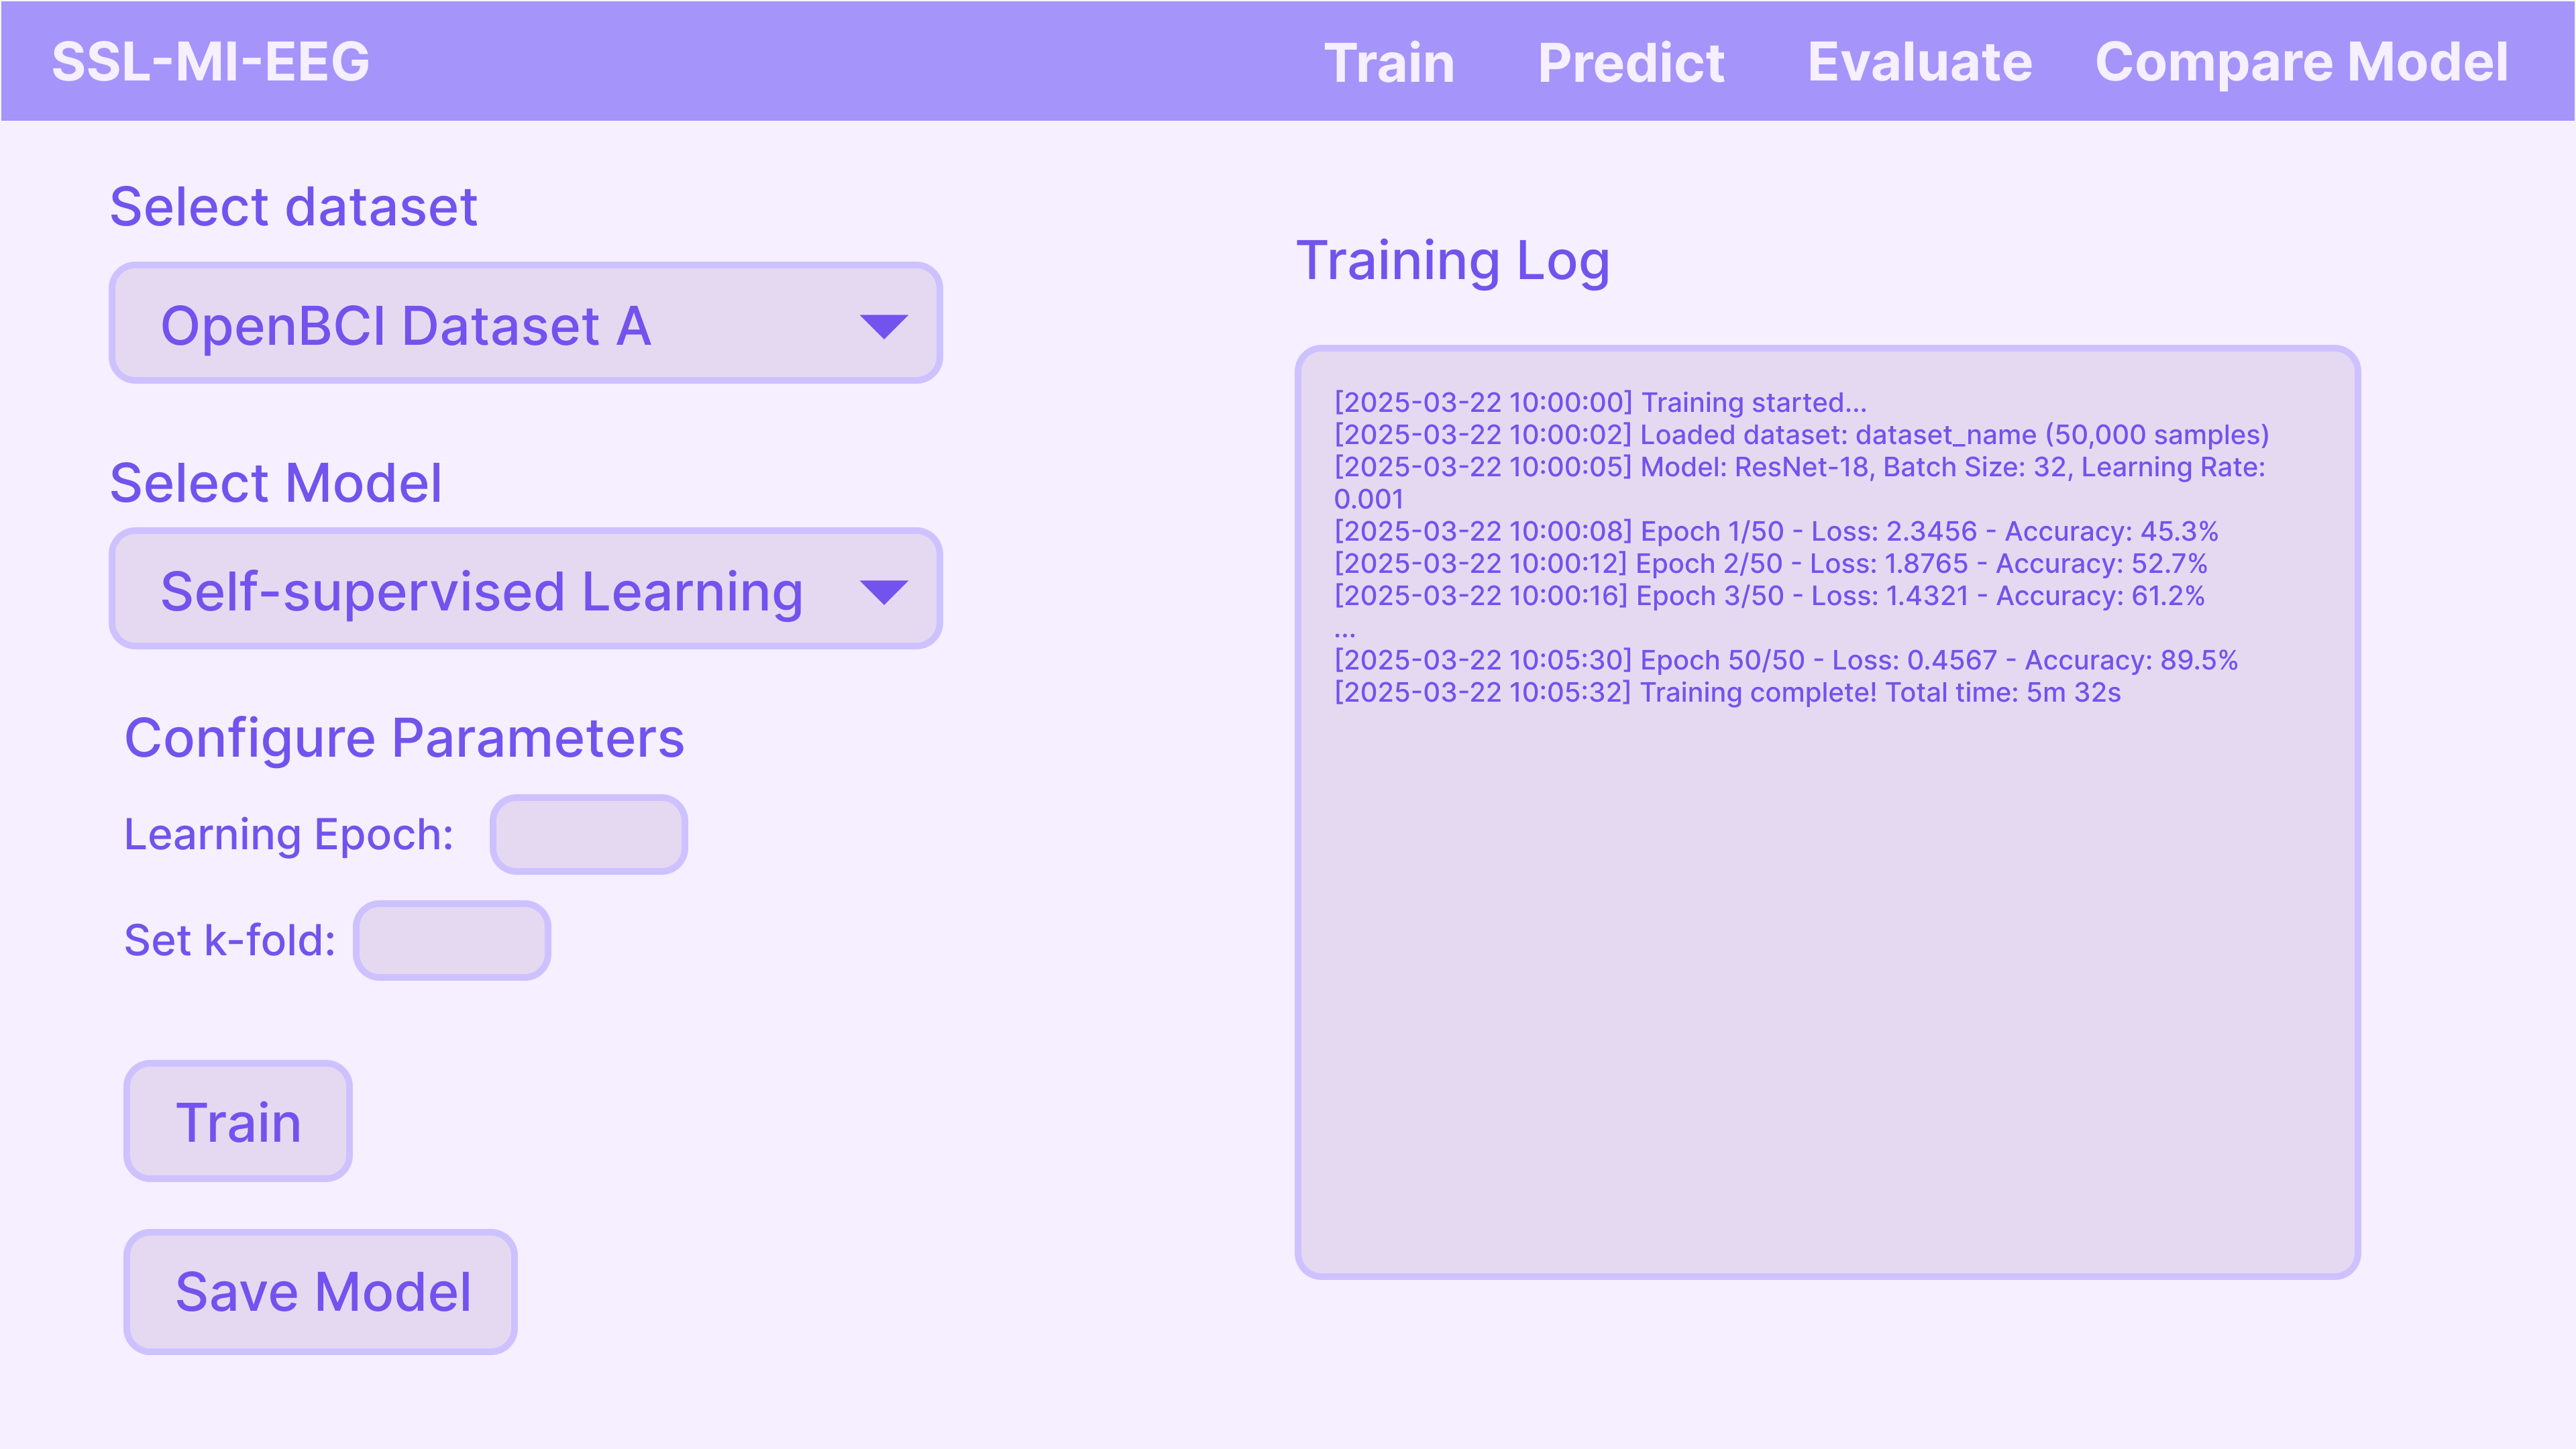
\includegraphics[width=0.9\textwidth]{figures/ui/train_model}
    \caption{Training Interface – Dataset selection, SSL configuration, and training log}
    \label{fig:figure2}
\end{figure}

\begin{figure}[h]
    \centering
    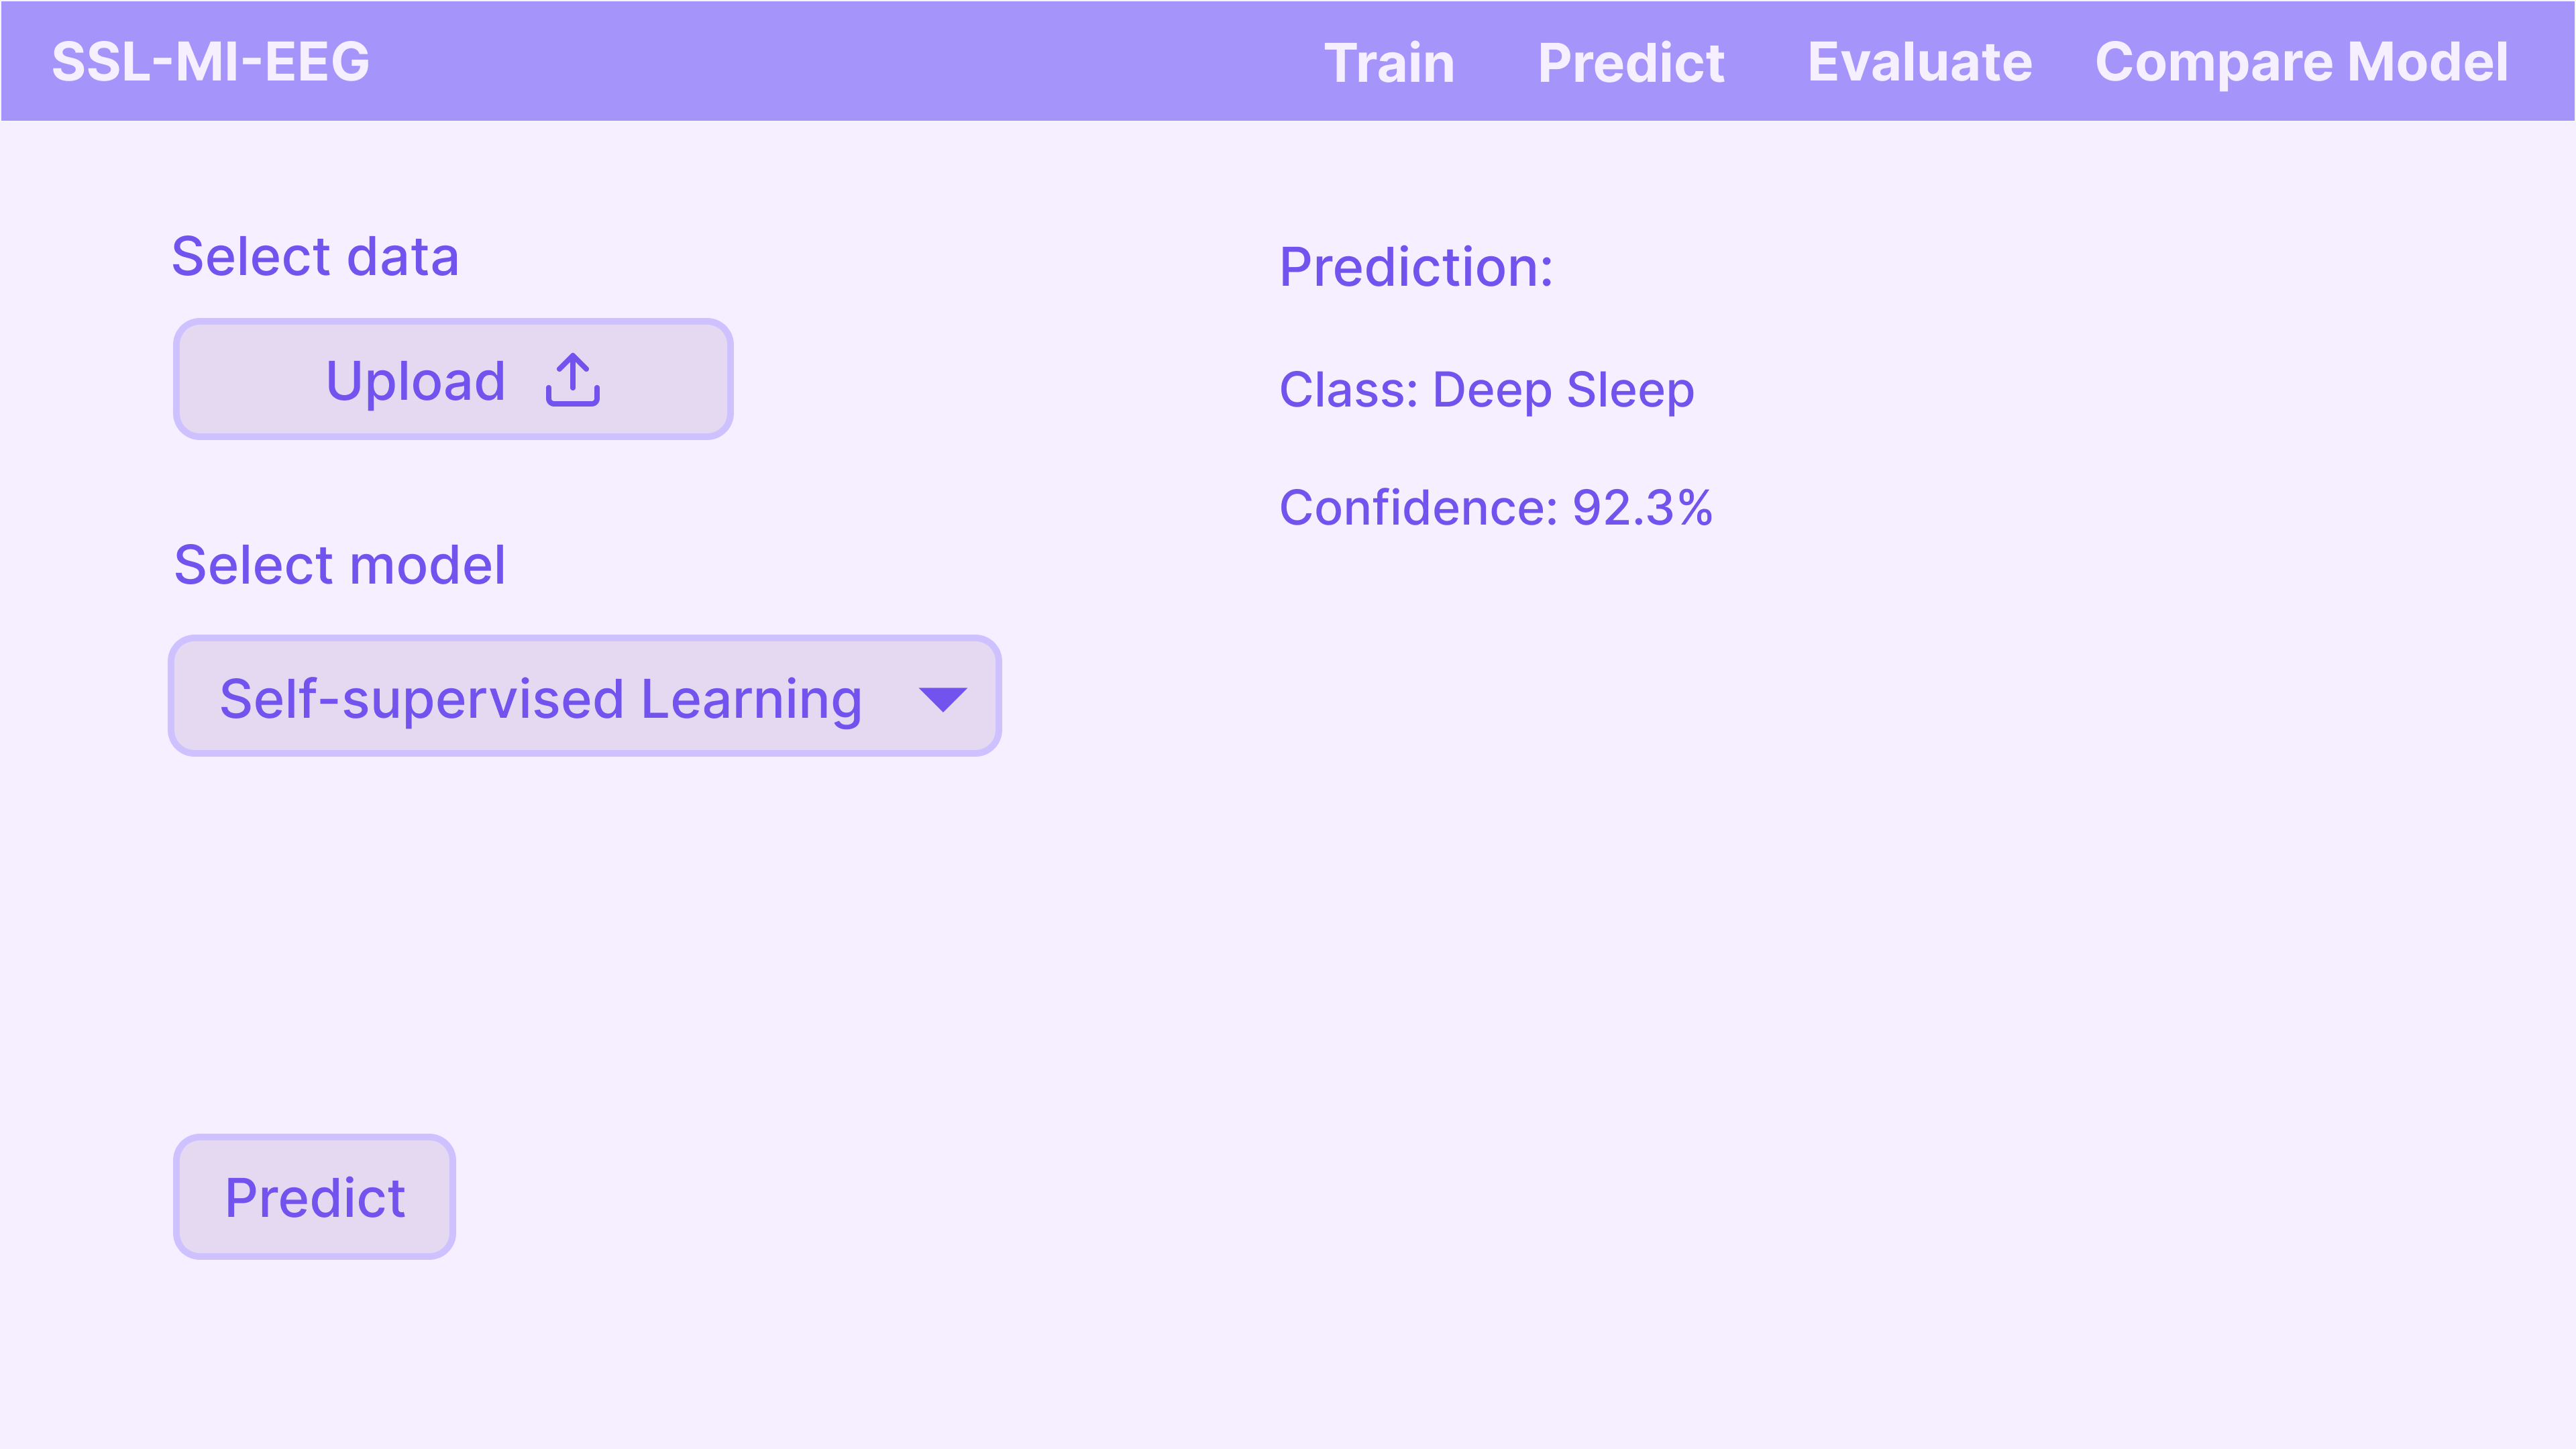
\includegraphics[width=0.9\textwidth]{figures/ui/predict_model}
    \caption{Prediction Interface – Uploading input data and viewing output class with confidence}
    \label{fig:figure3}
\end{figure}

\begin{figure}[h]
    \centering
    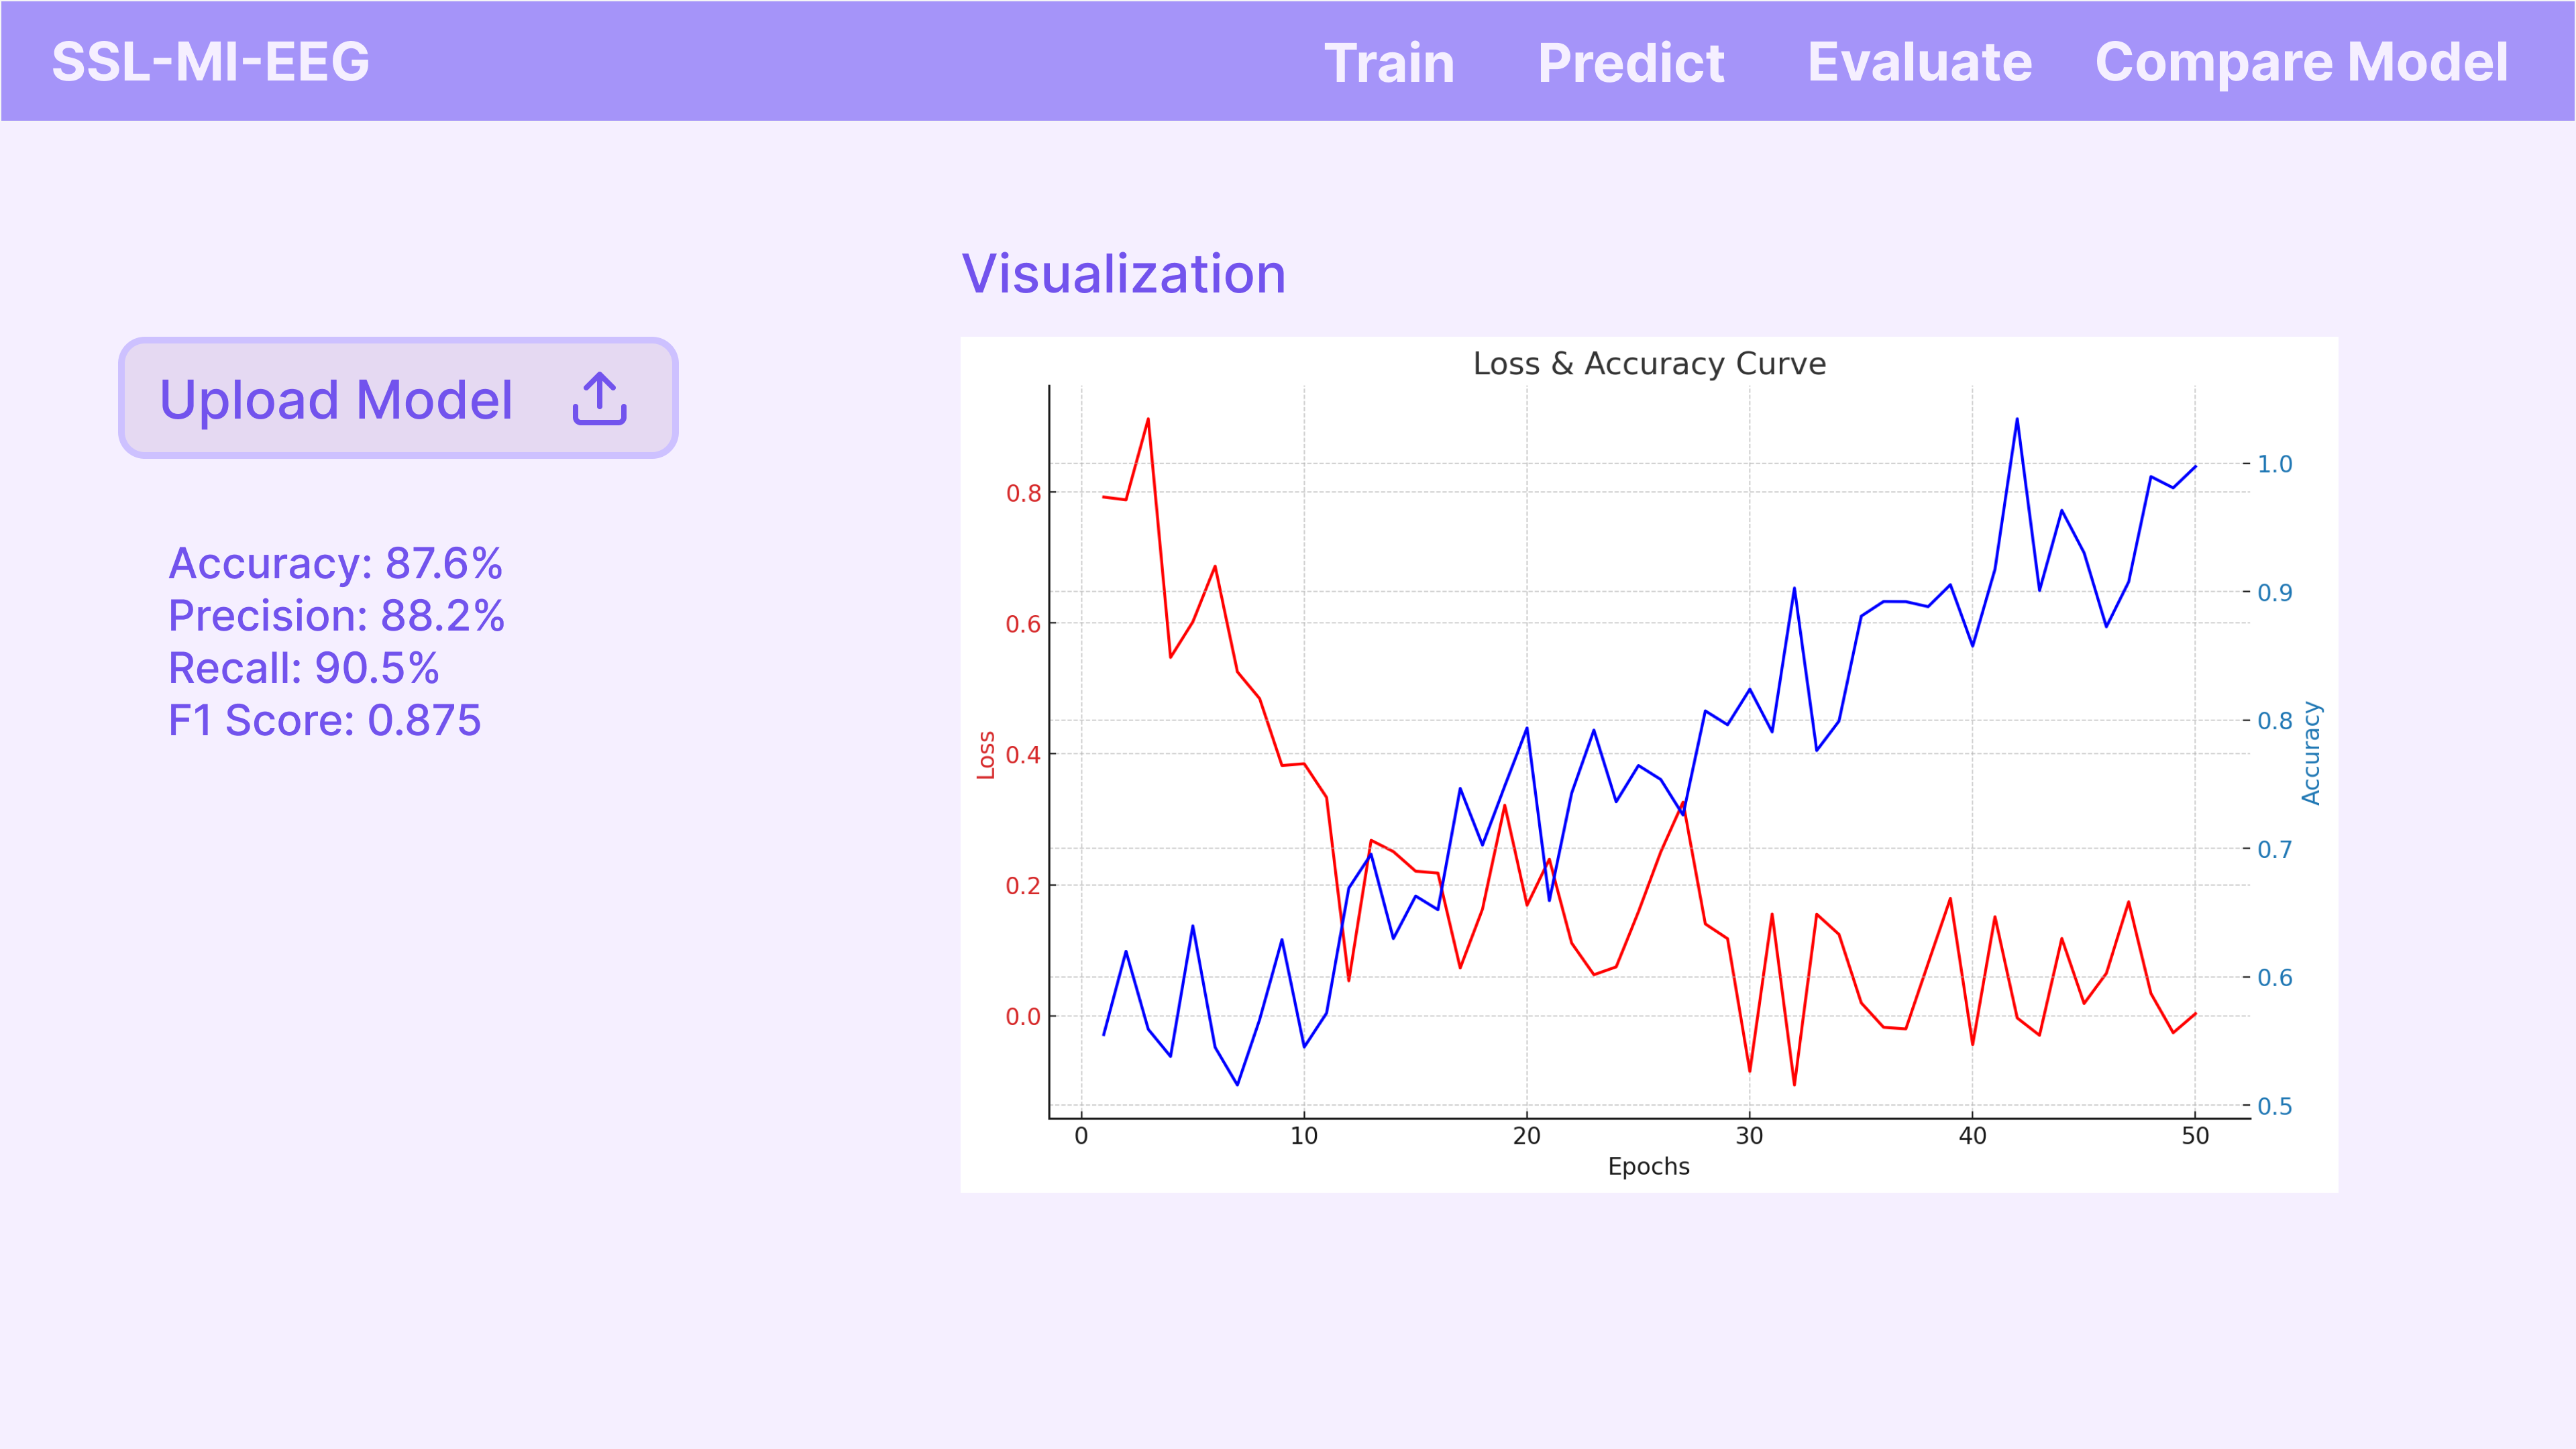
\includegraphics[width=0.9\textwidth]{figures/ui/evaluate_model}
    \caption{Evaluation Interface – Upload trained model and view performance metrics and curve}
    \label{fig:figure4}
\end{figure}

\begin{figure}[h]
    \centering
    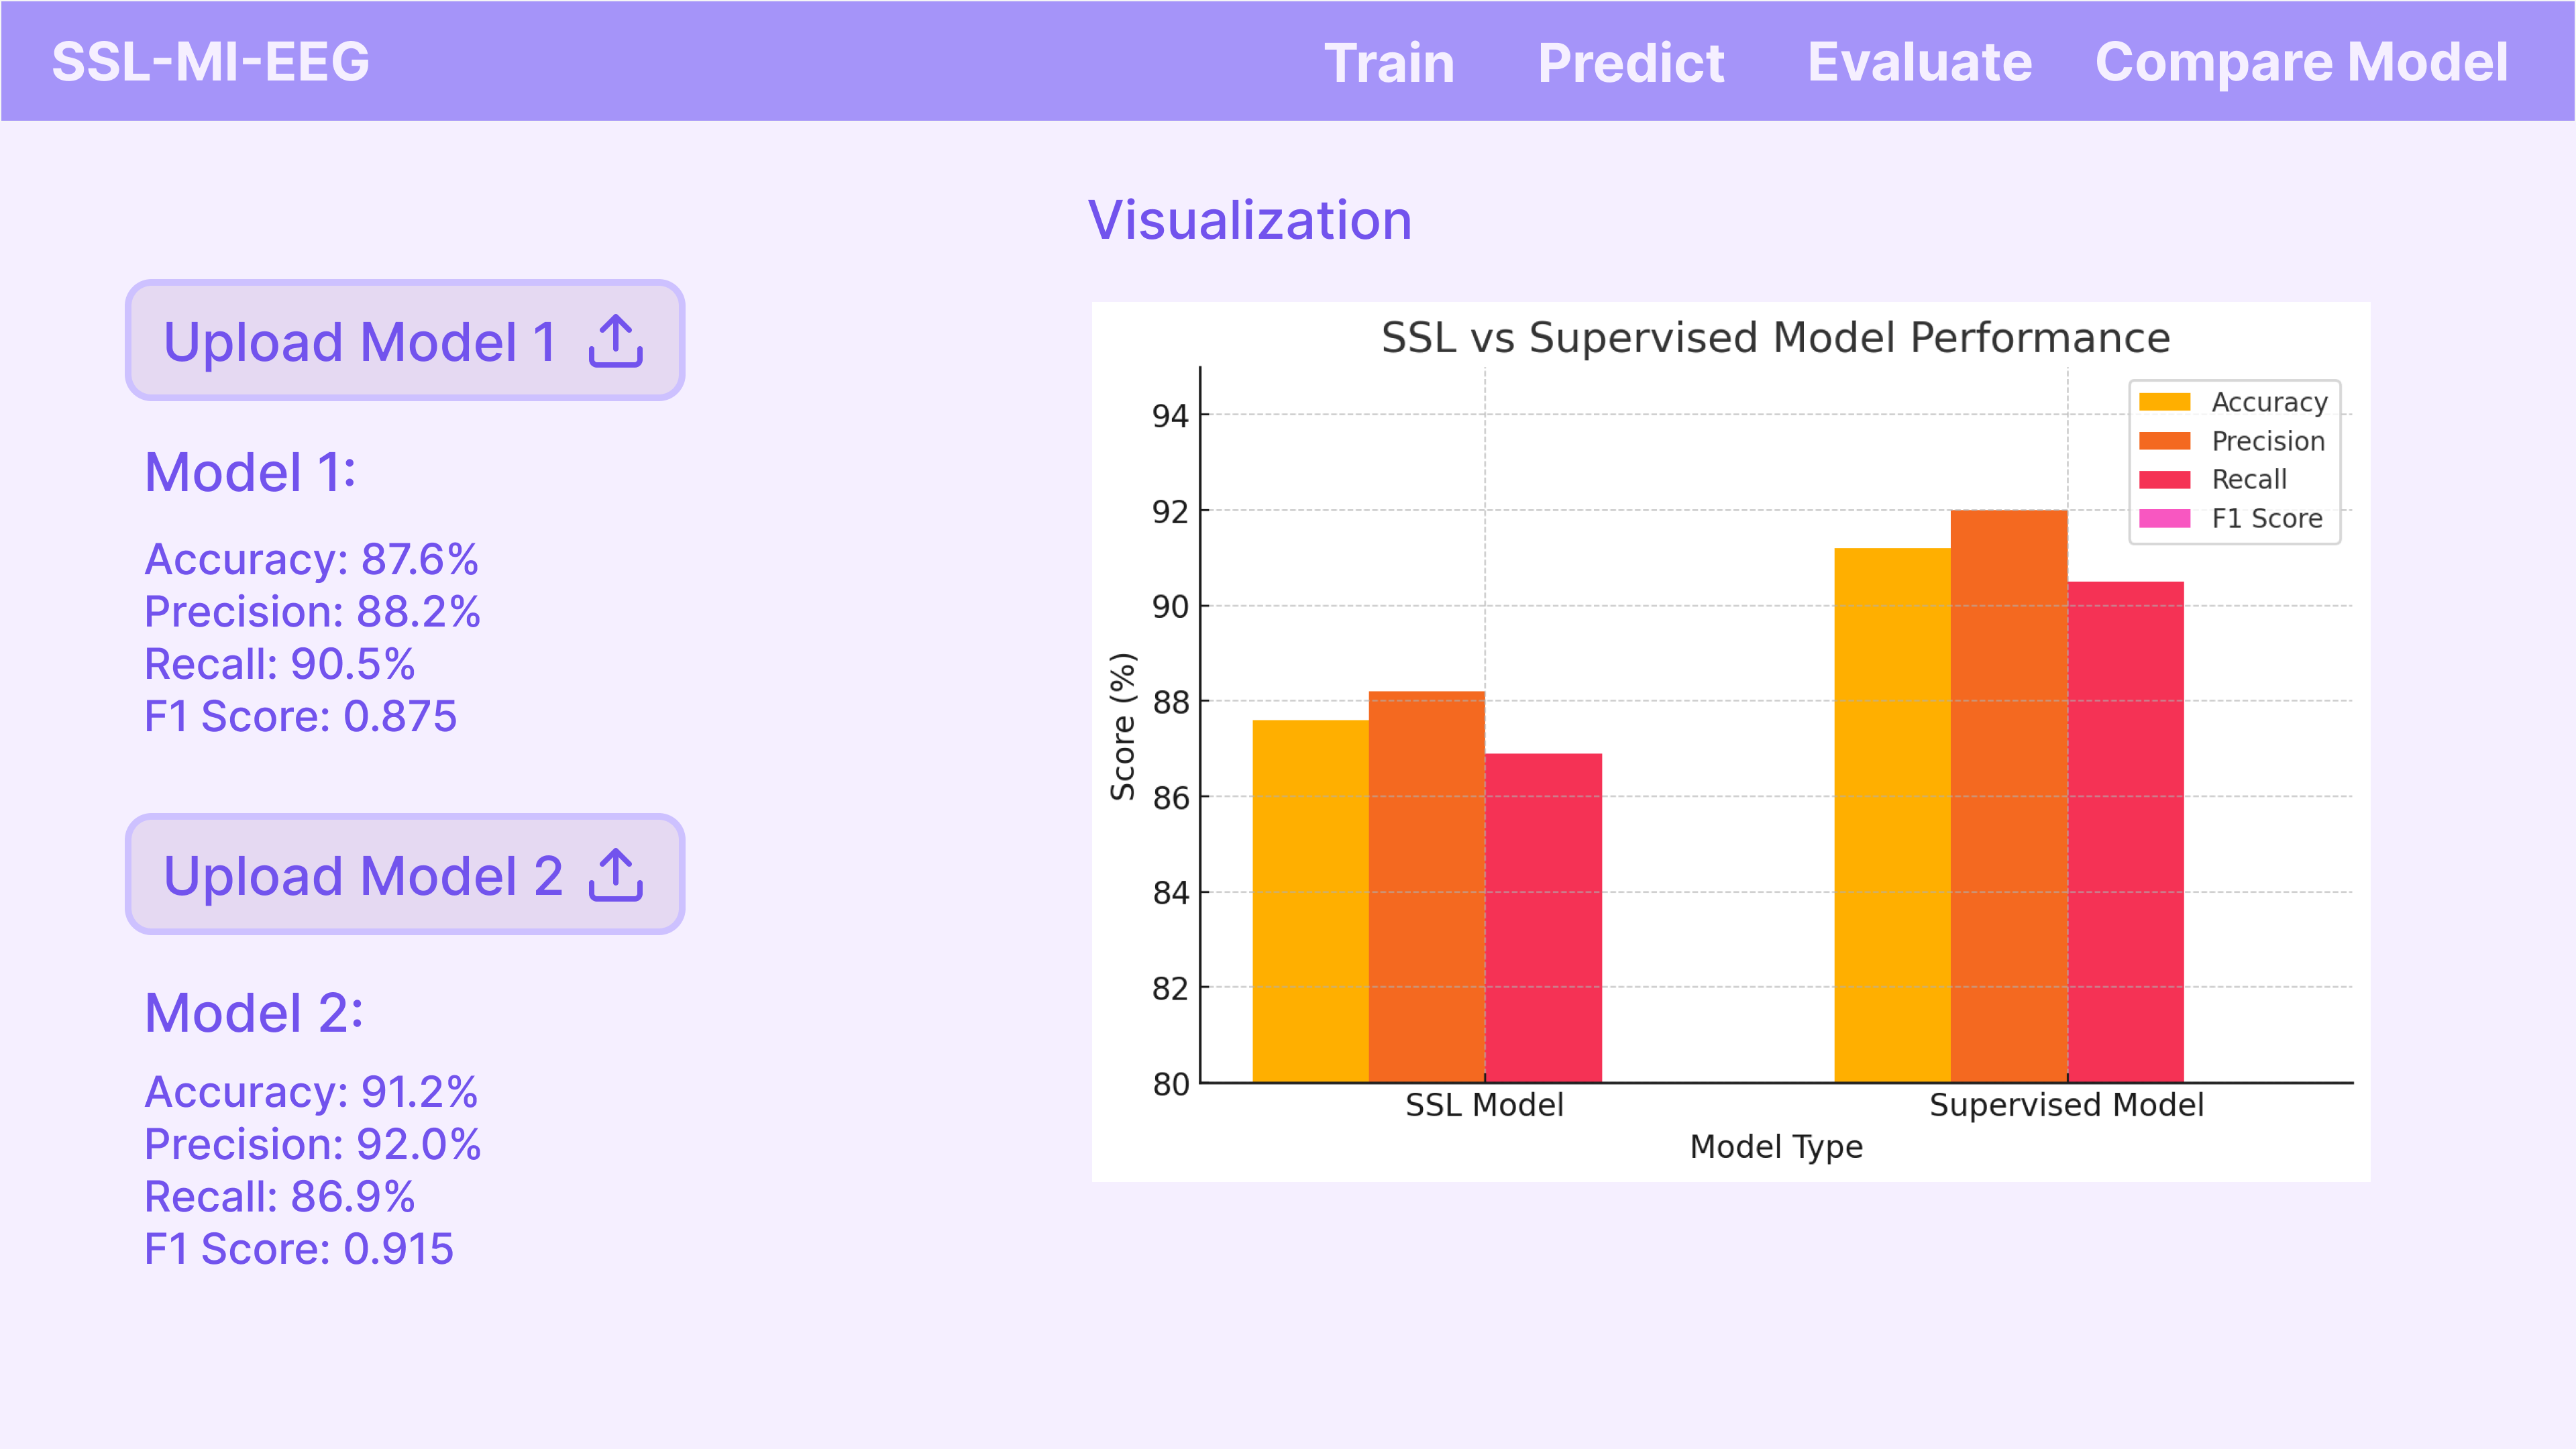
\includegraphics[width=0.9\textwidth]{figures/ui/compare_model}
    \caption{Comparison Interface – Visual comparison between SSL and Supervised models}
    \label{fig:figure5}
\end{figure}

